\documentclass[a4paper]{article}
\usepackage[procnames]{listings}
\usepackage{color}
\usepackage{graphicx}

\begin{document}
\definecolor{keywords}{RGB}{255,0,90}
\definecolor{comments}{RGB}{0,0,113}
\definecolor{red}{RGB}{160,0,0}
\definecolor{green}{RGB}{0,150,0}
\lstset{language=Python, 
        basicstyle=\ttfamily\small, 
        keywordstyle=\color{keywords},
        commentstyle=\color{comments},
        stringstyle=\color{red},
        showstringspaces=false,
        identifierstyle=\color{green},
        procnamekeys={def,class}}

\title{Face Recognition}
\author{Bochen Wang}
\maketitle
\section*{Introduction}
This is the first part of Homework 2. SVD is used to do the dimension reduction. Logistic regression is used to classify the faces.
\section*{Implementation}
\subsection*{Read Data}
Read data from the downloaded files and store them into numpy arrays.
\begin{lstlisting}
# Part a and Part b Read Data
train_labels, train_data = [], []
for line in open('./faces/train.txt'):
    im = misc.imread(line.strip().split()[0])
    train_data.append(im.reshape(2500,))
    train_labels.append(line.strip().split()[1])
train_data, train_labels = np.array(train_data, dtype=float), 
	np.array(train_labels, dtype=int)
print train_data.shape, train_labels.shape
plt.imshow(train_data[11, :].reshape(50,50), cmap = cm.Greys_r)
plt.show()

test_labels, test_data = [], []
for line in open('./faces/test.txt'):
    im = misc.imread(line.strip().split()[0])
    test_data.append(im.reshape(2500,))
    test_labels.append(line.strip().split()[1])
test_data, test_labels = np.array(test_data, dtype=float), 
	np.array(test_labels, dtype=int)
\end{lstlisting}

\subsection*{Calculate the Mean}
Calculate the mean vector of all the training data.
\begin{lstlisting}
# Part c Calculate Mean
mu = np.sum(train_data,axis=0)
mu /= train_data.shape[0]
print mu
plt.imshow(mu.reshape(50,50),cmap = cm.Greys_r)
plt.show()
\end{lstlisting}
Show the mean picture of train data.

\includegraphics{Mean.png}

\subsection*{Subtract Mean Vector}
Subtract the mean vector from all the train data vectors and test data vectors.
\begin{lstlisting}
# Part d Subtract Mean
for i in range(train_data.shape[0]):
    train_data[i] = train_data[i] - mu
plt.imshow(train_data[10, :].reshape(50,50), cmap = cm.Greys_r)
for i in range(test_data.shape[0]):
    test_data[i] = test_data[i] - mu
plt.imshow(test_data[10, :].reshape(50,50), cmap = cm.Greys_r)
\end{lstlisting}

\subsection*{SVD}
Implement SVD on the train data matrix and extract the 10 eigenvectors corresponding to 10 biggest eigenvalues. 
\begin{lstlisting}
# Part e SVD
U, s, V = np.linalg.svd(train_data, full_matrices=False)
for i in range(10):
    plt.imshow(V[i].reshape(50,50), cmap = cm.Greys_r)
    plt.show()
    plt.imsave(str(i)+".png",V[i].reshape(50,50), cmap = cm.Greys_r)
\end{lstlisting}
And show these eigenvectors in picture.
\begin{enumerate}
	\item 
\includegraphics{1}
	\item 
\includegraphics{2}
	\item 
\includegraphics{3}
	\item 
\includegraphics{4}
	\item 
\includegraphics{5}
	\item 
\includegraphics{6}
	\item 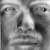
\includegraphics{7}
	\item 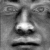
\includegraphics{8}
	\item 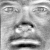
\includegraphics{9}
\end{enumerate}
\subsection*{Rank-r Approximation}
For r between 1 and 200, calculate the rank-r approximation error.
\begin{lstlisting}
# Part f rank-r approximation error
y_axis = []
x_axis = range(1,201)
for r in x_axis:
    sigma = np.zeros((r,r))
    for i in range(r):
        sigma[i][i] = s[i]
    U_r = U[:,:r]
    V_r = V[:r,:]
    X_r = np.mat(U_r) * np.mat(sigma) * np.mat(V_r)
    sub = train_data-X_r
    y_axis.append(np.linalg.norm(sub))

plt.plot(x_axis,y_axis)
plt.xlabel("r")
plt.ylabel("rank-r approximation error ")
#plt.savefig('rank-r_approximation_error.png')
plt.show()
\end{lstlisting}
Plot the histogram of rank-r approximation error and r.
\begin{center}
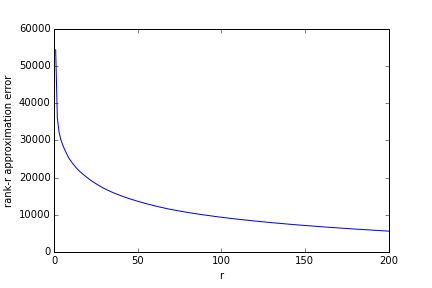
\includegraphics[scale = 0.7 ]{rank-r_approximation_error}	
\end{center}
\subsection*{Eigenface Feature}
Reduce the Feature dimension by reconstruct the train and test data with first r eigenvectors. 
\begin{lstlisting}
# Part g Eigenface feature
def eigenface(r):
    V_r = np.transpose(V[:r,:])
    F = np.mat(train_data) * np.mat(V_r)
    F_test = np.mat(test_data) * np.mat(V_r)
    return F,F_test
\end{lstlisting}
\subsection*{Face Recognition}
Implement logistic regression classification on the r-eigenvector based reconstructed data. 
\begin{lstlisting}
# Part h
F,F_test = eigenface(10)
logistic = linear_model.LogisticRegression()
logistic.fit(F,train_labels)
score = logistic.score(F_test,test_labels)
print score
# The accuracy with r = 10 is 0.79
y_axis = []
for r in x_axis:
    F,F_test = eigenface(r)
    logistic = linear_model.LogisticRegression()
    logistic.fit(F,train_labels)
    score = logistic.score(F_test,test_labels)
    y_axis.append(score)

plt.plot(x_axis,y_axis)
plt.xlabel("r")
plt.ylabel("classification accuracy")
#plt.savefig('classification_accuracy.png')
plt.show()
\end{lstlisting}
Plot the histogram of classification accuracy and r.
\begin{center}
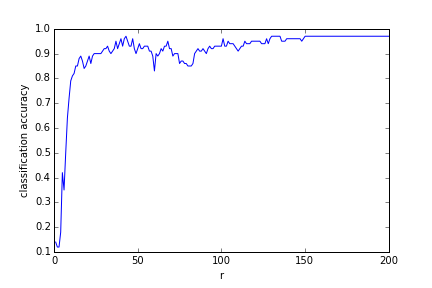
\includegraphics[scale = 0.6]{classification_accuracy}
\end{center}
\end{document}